\documentclass[10pt]{article}
\usepackage[letterpaper,margin=.75in]{geometry}
\usepackage[T1]{fontenc}
\usepackage{lmodern,amsmath,booktabs,graphicx}
\usepackage[hidelinks]{hyperref}
\setlength{\parskip}{4pt}
\setlength{\parindent}{0pt}
\begin{document}
{\Large\bfseries Forecasting LLM releases with a compound Poisson process}\par
{\small ISYE 4031, Group 1 \hfill November 17, 2026}\par
{\footnotesize AI assistance supported implementation, numerical checking, and drafting.}\par
{\small Rahul Mehta, Ishaan Mohan, Zhengyu Chris Liu, Timothy Kim, Chau M Duong}
\section*{Question and probability model}
We investigate whether a release forecast benefits from modeling joint announcements and changing arrival rates. The outcome is the number of benchmark-catalog models released over 42 days. This is the first stage of the group's adoption-forecasting pipeline. The section evaluates that stage on its own terms.

Poisson models are a natural starting point for counts over fixed exposures. We observe one-day intervals and retain days with zero releases. For an ordinary nonhomogeneous Poisson model, $Y_d\sim\operatorname{Poisson}(\lambda_d)$, with a time-varying mean such as
\[
 \log\lambda_d=\beta_0+\beta_1t_d+\beta_2W_d,
\]
where $t_d$ is years since January 1, 2024 and $W_d$ indicates Monday through Friday. Independent increments and equality of the conditional mean and variance are substantive assumptions. Several versions of a model may be announced together, creating a reason to test a different event unit.

We define a batch as models from the same provider on the same day. Let $B_d\sim\operatorname{Poisson}(\nu_d)$ count batches and let $K_{dj}\geq1$ be models in batch $j$. The total is
\[
 Y_d=\sum_{j=1}^{B_d}K_{dj},\qquad
 E(Y_d)=\nu_d E(K),\qquad
 \operatorname{Var}(Y_d)=\nu_d E(K^2).
\]
This compound construction permits greater model-count variability while retaining a regression for the batch rate. The moments assume independent batch marks with a fixed distribution within the forecast window. The construction follows the batch-arrival formulation in the technical source \cite{compound}.

\section*{Data and experimental design}
The frozen October 30, 2026 Epoch AI snapshot has 221 scored model releases from January 2024 onward, forming 179 provider-day batches. Missing providers receive distinct placeholders. The target population is models selected for this scored catalog, whose scope can change over time \cite{epoch}.

We compare 12 prespecified-for-this-run candidates over six nonoverlapping 42-day windows from February 21 through October 30, 2026. They include constant and trending rates, weekday effects, empirical batch sizes, separate weekday indicators, a quadratic trend, shorter rate histories, and recent or provider-specific batch sizes.

The primary selection procedure chooses among nine compound candidates by mean count negative log probability on four earlier 42-day windows. It then refits before each outer window. Each inner window ends by its outer training cutoff. The six outer windows were examined in previous work, so this is a retrospective investigation, even though every fit respects temporal order. Individual candidate scores are descriptive comparisons rather than independent confirmation after model selection.
\newpage
\section*{Results and metric interpretation}
Count MAE is the average absolute error in the total number of models per 42 days. Count negative log loss is $-\log P(Y=y_{\rm observed})$, averaged over windows, and rewards probability assigned to the realized total. Lower values are preferable. We report 90\% interval coverage with interval width and the interval score
\[
 S=(U-L)+20(L-y)_+ +20(y-U)_+.
\]
This score penalizes both wide intervals and misses. All intervals condition on fitted rate parameters and empirical batch probabilities. Parameter-estimation and catalog uncertainty are excluded.

{\small
\setlength{\tabcolsep}{9pt}
\begin{tabular}{@{}lrrrrr@{}}
\toprule
Specification & MAE & Log loss & Coverage & Width & Interval score\\
\midrule
Constant model rate & 4.75 & 3.59 & 4/6 & 9.3 & 26.00 \\
Time trend & 3.38 & 2.96 & 5/6 & 10.7 & 14.00 \\
Time + weekday & 3.39 & 2.97 & 4/6 & 10.5 & 17.17 \\
Constant batch rate & 4.75 & 3.34 & 4/6 & 11.7 & 18.33 \\
Batches + time & 2.81 & 2.76 & 6/6 & 13.0 & 13.00 \\
Batches + time + weekday & 2.81 & 2.76 & 6/6 & 13.2 & 13.17 \\
Separate weekday indicators & 2.81 & 2.76 & 6/6 & 13.0 & 13.00 \\
Quadratic batch trend & 3.57 & 2.89 & 6/6 & 13.5 & 13.50 \\
365-day rate history & 4.58 & 3.12 & 5/6 & 14.3 & 17.67 \\
504-day rate history & 3.27 & 2.83 & 6/6 & 13.8 & 13.83 \\
Recent batch sizes & 3.12 & 2.86 & 6/6 & 12.2 & 12.17 \\
Provider-specific sizes & 2.78 & 2.74 & 6/6 & 13.2 & 13.17 \\
Earlier-window selection & 3.26 & 2.92 & 5/6 & 12.8 & 16.17 \\
\bottomrule

\end{tabular}
}

The constant-rate baseline misses by 4.75 models per window on average. A time trend with weekday effects lowers this to 3.39. Adding empirical batch sizes lowers it further to 2.81, a 17.1\% reduction against the weekday model, and improves five of six windows. Provider-specific sizes reach 2.78, a further reduction of only 0.04 models. This small gain warrants caution.

The selected procedure obtains MAE 3.26, a 4.0\% reduction against the weekday model, and wins three of six windows. It selects a constant batch rate for the first two windows and provider-specific sizes for the remaining four. The initial constant selections miss the later increase in release volume. This explains why temporal model selection performs worse than choosing the best candidate from all six results.

\begin{figure}[h]
\centering
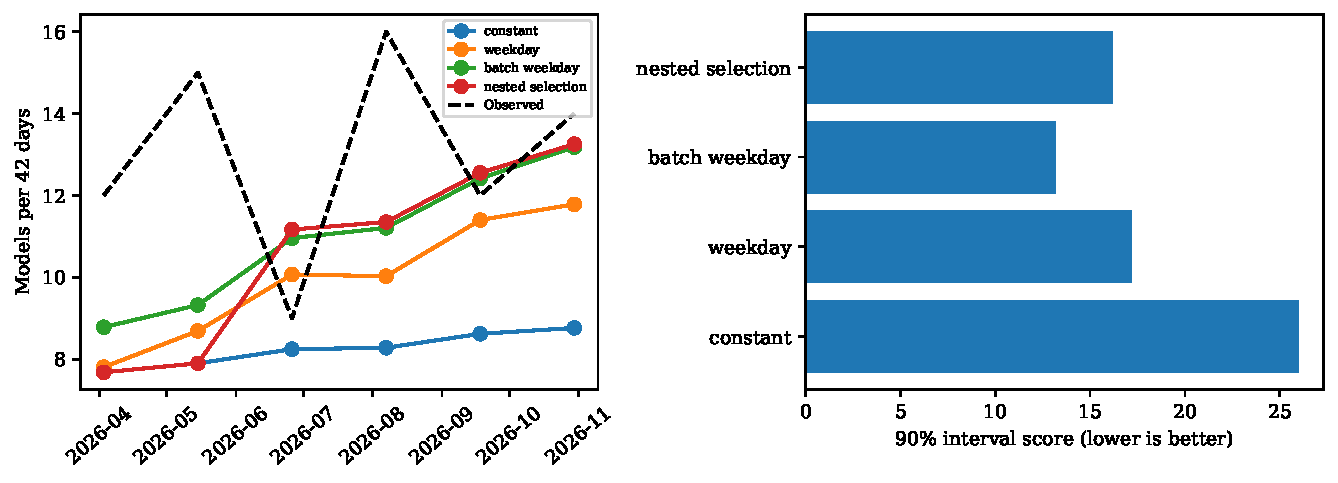
\includegraphics[width=.90\linewidth]{../../results/poisson_investigation/comparison.pdf}
\caption{Left, predicted and observed 42-day totals. Right, interval scores combine coverage and width. Earlier-window selection describes the executable selection rule.}
\end{figure}
\newpage
\section*{Why the results differ}
\textbf{Calendar timing and total counts.} Weekday effects lower daily log loss from 0.744 for the time-only model to 0.671, while total-count MAE changes from 3.38 to 3.39. Each window has six complete weeks. Allocating releases toward weekdays can improve their daily distribution without substantially changing the six-week total.

\textbf{Batching changes dispersion.} The weekday model expects 7.7 days with multiple model releases across the outer windows, compared with 16 observed. The compound weekday model expects 14.4 and the provider-size version expects 15.1. Both use earlier observations to estimate batch marks. Together with improved count log loss and interval scores, this supports batching as a useful statistical description of release variability.

\begin{figure}[h]
\centering
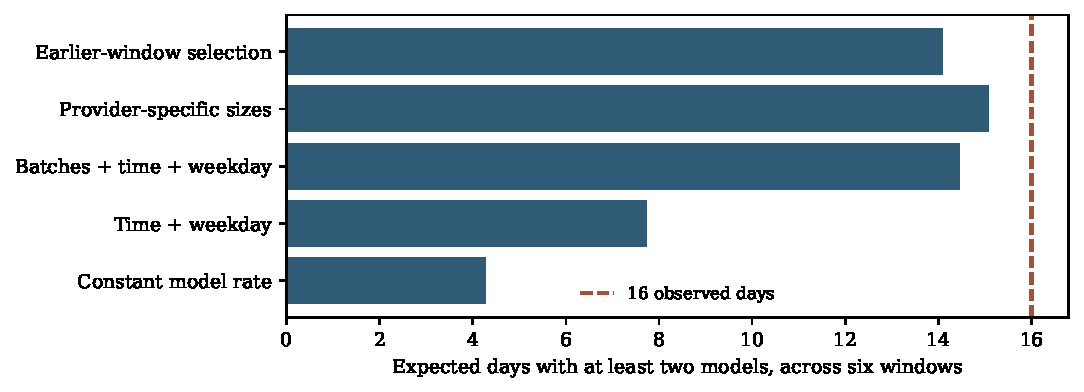
\includegraphics[width=.85\linewidth]{../../results/poisson_investigation/busy_days.pdf}
\caption{Expected busy days across the same six windows, compared with the observed total. Changing the batch event definition accounts for much of the discrepancy.}
\end{figure}

\textbf{Additional information and estimation noise.} Recent batch sizes use a 180-day sample shrunk toward the global distribution by 20 pseudo-batches. Provider-specific sizes use 10 pseudo-batches per provider, then weight provider distributions by recent batch shares shrunk with 20 global-share pseudo-batches. These fixed choices reduce instability for sparse providers. Provider effects concern batch size and mixture composition, rather than separate provider arrival-rate regressions.

Restricting rate estimation to 365 days worsens count MAE to 4.58, while 504 days gives 3.27. A quadratic trend gives 3.57. These comparisons show that the tested local-history and curvature specifications do not improve this sample's totals. Reduced information and unstable extrapolation are plausible explanations, but the comparisons do not isolate a unique cause.

\section*{Conclusion and handoff}
The compound weekday model is the clearest structural improvement in this retrospective sample. It reduces total-count error and represents busy days more closely. Provider-size refinement adds a small descriptive gain. Selection based entirely on earlier windows produces a smaller improvement, so the strongest defensible conclusion concerns the batch mechanism and its uncertainty representation, rather than a large established gain from tuning.

The adoption team should compare these first-stage predictions with direct adoption forecasts on identical observations. Improved release-count forecasts alone do not establish an adoption benefit. Independent batch arrivals, stationary batch marks within a window, catalog selection, and only six evaluated windows remain limitations. Later observations and further checks of forecast stability are required.

{\footnotesize
\begin{thebibliography}{9}
\bibitem{compound} P. Xu. \emph{Order Fill Rate, Leadtime Variability, and Advance Demand Information}. MIT OpenCourseWare, 2004, slide 3. \href{https://ocw.mit.edu/courses/15-764-the-theory-of-operations-management-spring-2004/7e65b5f67ebdb735f55d984413f56b84_lec7_xu.pdf}{Technical notes}.
\bibitem{epoch} Epoch AI. \href{https://epoch.ai/data/eci-documentation/methodology}{\emph{Epoch Capabilities Index documentation}}. Frozen scores retrieved October 30, 2026.
\end{thebibliography}
}
\end{document}
